\documentclass[../main.tex]{subfile}

\begin{document}

\section{Алгебраические методы интерполирования}
Задача интерполирования функции состоит в том, чтобы по известным её значениям
в некоторых точках определить её значения в остальных точках области задания.
Такая задача возникает, например, когда по результатам измерения некоторой
физической величины в одних точках требуется определить её значения в других
точках или когда в целях ускорения вычислений желательно приблизить заданную
функцию более лёгкой в вычислении. Как правило, интерполируют полиномами.

\begin{define}\label{eq:interpolating_polynomial}
	Алгебраический полином $P_m(x)=\sum_{k=0}^{m}a_kx^k$ называется
	\textbf{интерполяционным} для функции $f(x)$, заданной на отрезке
	$[a,b]$ по её значениям $f(x_i)$ в $n+1$ попарно различных точках
	$x_i\in[a,b]$ (\textbf{узлах интерполяции}), если
	\[\forall i\in\{0,1,...,n\}\;P_m(x_i)=f(x_i).\]
\end{define}

\begin{define}\label{eq:interpolation_problem}
	\textbf{Задача алгебраической интерполяции} -- построить алгебраический
	полином, который удовлетворял бы условию
	\eqref{eq:interpolating_polynomial}. Далее будем писать просто ЗАИ.
\end{define}

Первый вопрос: а какие условия гарантируют существование и единственность
интерполяционного многочлена? Для $m+1$ неизвестного члена полинома мы имеем
$n+1$ условие. Единственность решения математических конечномерных задач
обычно обеспечивается равенством числа неизвестных числу условий. В противном
случае, мы можем либо получить несколько решений, либо не получить их вовсе.

\begin{theorem}[о существовании и единственности интерполяционного многочлена]
\label{eq:polynominal_theorem}
	ЗАИ при $n=m$ имеет единственное решение.
\end{theorem}

\beginproof

	Запишем систему в матричном виде:
	\[
	\begin{pmatrix}
		1	& x_0	& x_0^2	& ...	& x_0^n \\
		1	& x_1	& x_1^2	& ...	& x_1^n \\
		...	& ...	& ...	&\ddots	& ...	\\
		1	& x_n	& x_n^2	& ...	& x_n^n \\
	\end{pmatrix}
	\begin{pmatrix}
		a_0 \\
		a_1 \\
		... \\
		a_n \\
	\end{pmatrix}
	=
	\begin{pmatrix}
		f(x_0)	\\
		f(x_1)	\\
		...	\\
		f(x_n)	\\
	\end{pmatrix}
	\]

	Определитель этой матрицы -- определитель Вандермонда -- не равен нулю,
	так как $x_i\ne x_j$ при $i\ne j$. Это необходимо и достаточно для
	существования и единственности решения.\qed

\subsection{Интерполяционный многочлен Лагранжа}
В теореме \eqref{eq:polynominal_theorem}, мы доказали, что решение ЗАИ
существует, но там не было ни слова о том, как его искать. Считать методом
Крамера -- слишком долго, чтобы не наскучило. Один из способ определить
интерполяционный полином предложил Луи Лагранж.

\begin{theorem}[о представлении в форме Лагранжа]\label{eq:lagrange_polynomial}
	При $n=m$ решение ЗАИ \eqref{eq:interpolation_problem} представимо в
	\textbf{форме Лагранжа}:
	\[P_n(x)=\sum_{k=0}^{n}\frac{\omega(x)}{(x-x_k)\omega'(x_k)}f(x_k),\]
	где
	\[\omega(x)=\prod_{l=0}^{n}(x-x_l).\]
\end{theorem}

\beginproof

	Для каждого $k\in\{0,1,...,n\}$ рассмотрим частный случай ЗАИ:
	\[P_{n,k}(x_i)=\delta_{k,i},\;i\in\{0,1,...,n\},\]
	где $\delta_{k,i}$ -- символ Кронекера. Так как полином $P_{n,k}$
	степени $n$ по условию имеет $n$ корней $\{x_0, x_1, ..., x_{k-1},
	x_{k+1}, ..., x_n\}$, он может быть представлен в виде произведения
	мономов:
	\[P_{n,k}(x)=q_k\prod_{\substack{l=0\\ l\neq k}}^{n}(x-x_l),\]
	где $q_k$ берётся из условия $P_{n,k}(x_k)=1$:
	\[q_k=\frac{1}{\prod_{\substack{l=0\\ l\neq k}}^{n}(x-x_l)}.\]
	Обозначив $\omega(x)=\prod_{l=0}^{n}(x-x_l)$, перепишем многочлен:
	\[P_{n,k}(x)=\frac{\omega(x)}{(x-x_k)\omega'(x_k)}f(x_k).\]
	Очевидно, что линейная комбинация
	\[P_n(x)=\sum_{k=0}^{n}P_{n,k}(x)f(x_k)\]
	полиномов -- многочлен степени $n$. А так как $\forall i\in\{0,...,n\}$
	\[P_n(x_i)=\sum_{k=0}^{n}P_{n,k}(x_i)f(x_k)=\sum_{k=0}^{n}\delta_{i,k}
	f(x_k)=f(x_i),\]
	полином является интерполянтом функции $f(x)$.\qed

\begin{example}
	Найдём интерполяционный многочлен Лагранжа функции \\ $f(x)=\cos x +
	\frac{x}{2}$ на отрезке $[0,4]$. Вот список значений:\newline

	\begin{tabular}{|c|c|c|c|}
		\hline
		$x$	& 0	& 2	& 4	\\
		\hline
		$f(x)$	& 1	& 0.584	& 1.346	\\
		\hline
	\end{tabular}

	\[\omega(x)=x(x-2)(x-4).\]

	\[P_2(x)=\omega(x)\Big (\frac{1}{8x}-\frac{0.584}{4(x-2)}
	+\frac{1.346}{8(x-4)} \Big )=\]
	\[=0.125(x^2-6x+8)-0.146(x^2-4x)+0.168(x^2-2x)=\]
	\[=0.149x^2-0.502x+1.\]

	Найдём значения некоторых внутренних точек:\newline

	\begin{tabular}{|c|c|c|}
		\hline
		$x$     & 1     & 3     \\
		\hline
		$f(x)$  & 1.04	& 0.51	\\
		\hline
		$P_2(x)$& 0.645	& 0.818	\\
		\hline
	\end{tabular}\newpage

	И изобразим всё это на графике:\newline

	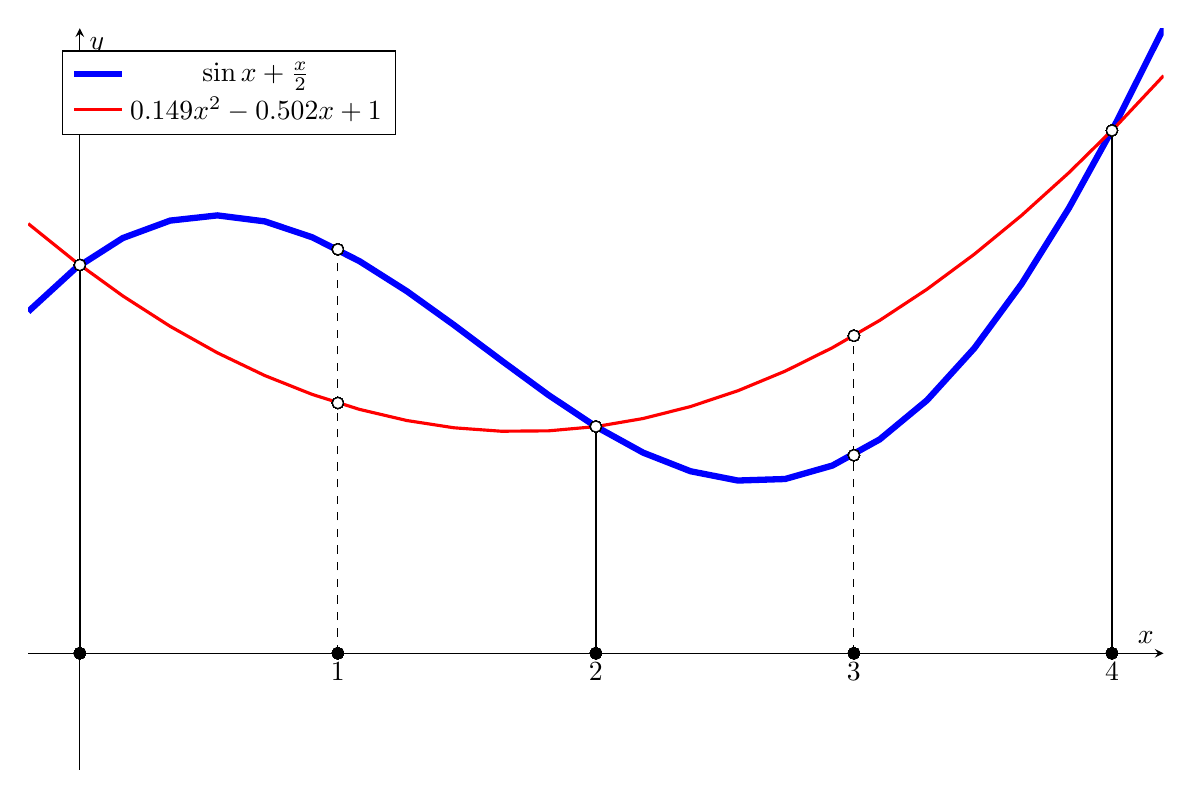
\begin{tikzpicture} [
		declare function= {
			u(\x) = cos(\x / pi * 180) + \x/2;
			subpolynonominal(\x,\A,\b,\c) = (\x-\b)*(\x-\c) /
				((\A-\b)*(\A-\c)) * u(\A);
			lag(\x,\a,\b,\c) =
				subpolynonominal(\x,\a,\b,\c) +
				subpolynonominal(\x,\b,\c,\a) +
				subpolynonominal(\x,\c,\a,\b);
		},]
		\begin{axis} [
			height=11cm,
			width=16cm,
			xlabel = {$x$},
			ylabel = {$y$},
			axis x line = middle,
			axis y line = middle,
			ymin = -0.3,
			domain = -0.2:4.2,
			ticks = none,
			legend pos = north west ]

			\newcommand*{\varA}{0}
			\newcommand*{\varB}{2}
			\newcommand*{\varC}{4}
			\newcommand*{\queryA}{1}
			\newcommand*{\queryB}{3}
			\pgfmathsetmacro{\fa}{u(\varA)}
			\pgfmathsetmacro{\fb}{u(\varB)}
			\pgfmathsetmacro{\fc}{u(\varC)}
			\pgfmathsetmacro{\Rfirst}{lag(\queryA,\varA,\varB,
				\varC)}
			\pgfmathsetmacro{\Rsecond}{lag(\queryB,\varA,\varB,
				\varC)}
			\pgfmathsetmacro{\RfirstTrue}{u(\queryA)}
			\pgfmathsetmacro{\RsecondTrue}{u(\queryB)}

			\addplot[color=blue, line width=.08cm]{u(x)};
			\addplot[color=red, line width=.04cm]{lag(x,\varA,
				\varB,\varC)};

			\coordinate(A) at 	(\varA,		\fa);
			\coordinate(Ap) at	(\varA,		0);
			\coordinate(B) at 	(\varB,		\fb);
			\node[below](Bp) at	(\varB,		0) {$\varB$};
			\coordinate(C) at 	(\varC,		\fc);
			\node[below](Cp) at	(\varC,		0) {$\varC$};
			\coordinate(Q1) at 	(\queryA,	\Rfirst);
			\node[below](Q1p) at	(\queryA,	0) {$\queryA$};
			\coordinate(Q1true) at	(\queryA,	\RfirstTrue);
			\coordinate(Q2) at 	(\queryB,	\Rsecond);
			\node[below](Q2p) at	(\queryB,	0) {$\queryB$};
			\coordinate(Q2true) at	(\queryB,	\RsecondTrue);

			\addplot[mark=*,only marks, fill=white] (\varA,\fa)
				node[above, pos=1]{};
			\addplot[mark=*,only marks, fill=white] (\varB,\fb)
				node[above, pos=1]{};
			\addplot[mark=*,only marks, fill=white] (\varC,\fc)
				node[above, pos=1]{};
			\addplot[mark=*,only marks, fill=white] (\queryA,\Rfirst)
				node[above, pos=1]{};
			\addplot[mark=*,only marks, fill=white] (\queryA,\RfirstTrue)
				node[above, pos=1]{};
			\addplot[mark=*,only marks, fill=white] (\queryB,\Rsecond)
				node[above, pos=1]{};
			\addplot[mark=*,only marks, fill=white] (\queryB,\RsecondTrue)
				node[above, pos=1]{};
			\addplot[mark=*,only marks, fill=black] (\varA,0)
				node[above, pos=1]{};
			\addplot[mark=*,only marks, fill=black] (\varB,0)
				node[above, pos=1]{};
			\addplot[mark=*,only marks, fill=black] (\varC,0)
				node[above, pos=1]{};
			\addplot[mark=*,only marks, fill=black] (\queryA,0)
				node[above, pos=1]{};
			\addplot[mark=*,only marks, fill=black] (\queryB,0)
				node[above, pos=1]{};

			\draw[thick] (Ap) -- (A)	(Bp) -- (B)
				(Cp) -- (C);
			\draw[dashed] (Q1p) -- (Q1true)	(Q2p) -- (Q2);

			\addlegendentry{$\sin x+\frac{x}{2}$};
			\addlegendentry{$0.149x^2-0.502x+1$};
		\end{axis}
	\end{tikzpicture}
\end{example}

\subsection{Интерполяционный многочлен Ньютона}
Предположим, что мы по $n+1$ узлам интерполяции построили полином Лагранжа
$P_n(x)$ для функции $f(x)$. Затем нам стало известно новое значение
интерполяционной функции при $x_{n+1}$. Вопрос: как быстро мы сможем перестроить
полином под новый узел интерполяции? От полинома $P_n(x)$ построить $P_{n+1}(x)$
нереально сложно, так как из \eqref{eq:lagrange_polynomial} придётся пересчитать
все ''коэффициенты'' вида \[\frac{\omega(x)}{(x-x_k)\omega'(x_k)}.\]

Надо найти новую запись интерполяционного многочлена. Заметьте -- именно запись,
так как по теореме \eqref{eq:polynominal_theorem} интерполяционный полином
единственнен.

\begin{define}\label{eq:divided_difference}
	\textbf{Разделённая разность $n$-го порядка} функции $f(x)$ на попарно
	разных узлах $x_0,...,x_n$ -- это число
	\[f[x_0,..., x_{n}]=\frac{f[x_1,...,x_n]-f[x_0,...,x_{n-1}]}
	{x_n-x_0},\]
	где $f[y_0,...,y_{n-1}]$ -- разделённая разность $n-1$ порядка, а
	разделённая разность первого порядка равна
	\[\boxed{f[x_0,x_1]=\frac{f(x_1)-f(x_0)}{x_1-x_0}}.\]
\end{define}

\begin{lemma}\label{eq:div_diff_formula}
	Для разделённой разности $n$-го порядка справедлива формула
	\[f[x_0,...,x_n]=\sum_{i=0}^{n}\frac{f(x_i)}
	{\prod_{\substack{j=0\\ j\neq i}}^{n}(x_i-x_j)}.\]
\end{lemma}

\beginproof

	Доказывать мы будем методом математической индукции. Для $n=1$ верность
	леммы очевидна для разделённой разности первого порядка.

	Теперь положим, что лемма верна при $n=m$. Докажем лемму для $m+1$.
	\[f[x_0,...,x_{m+1}]=\frac{f[x_1,...,x_{m+1}]-f[x_0,...,x_m]}
	{x_{m+1}-x_m}=\]
	\[{\overset{\substack{\text{инд.}\\\text{предп.}}}{=\joinrel=}}
	\frac{1}{x_{m+1}-x_0}\Big( \sum_{i=1}^{m+1}\frac{f(x_i)}
	{\prod_{\substack{j=1\\ j\neq i}}^{m+1}(x_i-x_j)} - \sum_{k=0}^{m}
	\frac{f(x_k)}{\prod_{\substack{l=0\\ k\neq l}}^{m}(x_k-x_l)}\Big)=\]
	\[=\frac{f(x_0)}{\prod_{i=1}^{m+1}(x_0-x_i)} + \frac{1}{x_{m+1}-x_0}
	\sum_{i=1}^{m} \Big(\frac{f(x_i)}{\prod_{\substack{j=1\\ j\neq i}}^
	{m+1}(x_i-x_j)}-\]
	\[-\frac{f(x_i)}{\prod_{\substack{j=0\\ j\neq i}}^{m}(x_i-x_j)}
	\Big) + \frac{f(x_{m+1})}{\prod_{i=0}^{m}(x_{m+1}-x_i)}. \tag{*}\]

	Преобразуем выражение, которое стоит внутри оператора суммы:
	\[\frac{f(x_i)}{\prod_{\substack{j=1\\ j\neq i}}^{m+1}(x_i-x_j)}-
	\frac{f(x_i)}{\prod_{\substack{j=0\\ j\neq i}}^{m}(x_i-x_j)}=\]
	\[=\frac{f(x_i)\big((\cancel{x_i}-x_0)-(\cancel{x_i}-x_{m+1})\big)}
	{\prod_{\substack{j=0\\ j\neq i}}^{m+1}(x_i-x_j)}=
	\frac{f(x_i)(x_{m+1}-x_0)}{\prod_{\substack{j=0\\ j\neq i}}^{m+1}
	(x_i-x_j)},\]

	И окончательно из (*) получим:
	\[f[x_0,...,x_n]=\frac{f(x_0)}{\prod_{i=1}^{m+1}(x_0-x_i)}+\sum_{j=1}^{m}
	\frac{f(x_j)}{\prod_{\substack{i=0\\ i\neq j}}^{m+1}(x_j-x_i)}+\]
	\[+\frac{f(x_{m+1})}{\prod_{i=0}^{m}(x_{m+1}-x_i)}=
	\sum_{i=0}^{m+1}\frac{f(x_i)}{\prod_{\substack{j=0\\ j\neq i}}^{m+1}
	(x_i-x_j)}.\qed\]

\begin{lemma}\label{eq:next_int_pol}
	Пусть $P_k(x)$ и $P_{k+1}(x)$ -- интерполяционные многочлены функции $f(x)$,
	тогда для них верно равенство:
	\[P_{k+1}(x)-P_k(x)=A_{k+1}\prod_{i=0}^{k}(x-x_k),\]
	где
	\[A_{k+1}=\frac{f(x_{k+1})-P_k(x_{k+1})}{\prod_{i=0}^{k}(x_{k+1}-x_i)}.\]
\end{lemma}

\beginproof

	Очевидно, что разность $P_{k+1}(x)-P_{k}(x)$ -- полином степени $k+1$.
	Также верно, что для первых $k+1$ интерполяционных узлов $P_{k+1}(x_i)=
	P_{k}(x_i)$. Поскольку у полинома степени $k+1$ ровно столько же нулей,
	верно разложение
	\[P_{k+1}(x)-P_{k}(x)=A_{k+1}\prod_{i=0}^{k}(x-x_i),\]
	где $A_{k+1}$ -- некоторая константа, которую можно найти из представления
	\[\underset{=f(x_{k+1})}{\underbrace{P_{k+1}(x_{k+1})}}-P_{k}(x_{k+1})=
	A_{k+1}\prod_{i=0}^{k}(x_{k+1}-x_i)\Rightarrow\]
	\[\Rightarrow \boxed{A_{k+1}=\frac{f(x_{k+1})-P_k(x_{k+1})}
	{\prod_{i=0}^{k}(x_{k+1}-x_i)}}.\qed\]

\begin{lemma}\label{eq:newton_koef_formula}
	Коэффициенты $A_k$ из леммы \eqref{eq:next_int_pol} равны разделённым
	разностям $k$-го порядка, то есть $A_k=f[x_0,...,x_k].$

\end{lemma}

\beginproof

	По формуле
	\[A_k=\frac{f(x_k)-P_{k-1}(x_k)}{\prod_{i=0}^{k-1}(x_k-x_i)}=
	\frac{f(x_k)}{\prod_{i=0}^{k-1}(x_k-x_i)} - \frac{P_{k-1}(x_k)}
	{\prod_{i=0}^{k-1}(x_k-x_i)}.\tag{*}\]

	Во втором слагаемом запишем полином $P_{k-1}(x_k)$ в форме\\Лагранжа
	\eqref{eq:lagrange_polynomial}:
	\[P_{k-1}(x)=\sum_{i=0}^{k-1}\frac{\omega(x)}{(x-x_i)\omega'(x_i)}
	f(x_i),\;\;
	\omega(x)=\prod_{j=0}^{k-1}(x-x_j).\]

	Заметим, что знаменатели в $(*)$ равны $\omega(x_k)$:
	\[A_k=\frac{f(x_k)}{\omega(x_k)} - \frac{1}{\cancel{\omega(x_k)}}
	\sum_{i=0}^{k-1}\frac{\cancel{\omega(x_k)}}{(x_k-x_i)\omega'(x_k)}
	f(x_i).\]
	И с учётом
	$\omega'(x_i)=\mathlarger\prod_{j=0,\;j\ne i}^{k-1}(x_i-x_j)$
	окончательно получаем:
	\[A_k=\frac{f(x_k)}{\prod_{j=0}^{k-1}(x_k-x_j)} +
	\sum_{i=0}^{k-1}\frac{f(x_i)}{\prod_{\substack{j=0\\j\ne i}}^{k-1}
	(x_i-x_j)}=\sum_{i=0}^{k}\frac{f(x_i)}{\prod_{\substack{j=0\\j\ne i}}^
	{k}(x_i-x_j)},\]
	что по лемме \eqref{eq:div_diff_formula} и является разделённой
	разностью $k$-го порядка на попарно разных узлах $x_0,...,x_k$.\qed

\begin{theorem}[о представлении в форме Ньютона]\label{eq:newton_polynomial}
	При $n=m$ решение ЗАИ \eqref{eq:interpolation_problem} представимо в
	\textbf{форме Ньютона}:
	\[\boxed{P_n(x)=\sum_{k=0}^{n}\big(f[x_0,...,x_k]\prod_{i=0}^{k-1}
	(x-x_i)\big)},\]
	где $f[x_0,...,x_k]$ -- разделённая разность $k$-го порядка
	\eqref{eq:divided_difference}.
\end{theorem}

\beginproof

	Данная теорема является следствием лемм \eqref{eq:next_int_pol} и
	\eqref{eq:newton_koef_formula}:
	\[P_n(x)=P_{n-1}(x)+A_n\prod_{k=0}^{n-1}(x-x_k)=...=
	\sum_{k=0}^{n}\big(A_k\prod_{i=0}^{k-1}(x-x_i)\big),\]
	в которой $A_k=f[x_0,...,x_k]$ и $A_0=f(x_0)$.\qed
\newpage

\subsection{Оценка погрешности интерполирования}
Третий и самый главный вопрос интерполирования -- насколько отличаются значения
интерполяционного многочлена $P_n(x)$ от значений интерполируемой функции $f(x)$?
Сначала дадим простое определение.

\begin{define}\label{eq:interpolation_error}
	\textbf{Погрешность} или \textbf{ошибка интерполирования} функции $f(x)$
	по её значениям $f(x_i)$ в попарно различных точках $x_0,...,x_n$
	интервала $[a,b]$ интерполяционным многочленом $P_n(x)$ -- это их
	разность $\boxed{R_n(x)=f(x)-P_n(x)}$.
\end{define}

То, что в узлах интерполяции погрешности нет -- это понятно. Нам бы хотелось
найти погрешность и в других точках.

\begin{lemma}\label{eq:interpolation_error_form}
	Если $y\in[a,b]\backslash\{x_0,...,x_n\}$, то
	\[R_n(y)=f[x_0,...,x_n,y]\omega(y),\quad
	\omega(y)=\prod_{k=0}^{n}(y-x_n).\]
\end{lemma}

\beginproof

	Построим новый интерполяционный полином $P_{n+1}(x)$ для $f(x)$ на
	$n+2$ попарно различных узлах $\{x_0,...,x_n,y\}$. Представим его в форме
	Ньютона \eqref{eq:newton_polynomial}:
	\[P_{n+1}(x)=P_n(x)+f[x_0,...,x_n,y]\omega(x)\Rightarrow\]
	\[\Rightarrow P_n(x)=P_{n+1}(x)-f[x_0,...,x_n,y]\omega(x).\]
	И тогда
	\[R_n(y)=f(y)-P_n(y)=\cancel{f(y)}-\cancel{P_{n+1}(y)}+f[x_0,...,x_n,y]
	\omega(y)\Rightarrow\]
	\[\Rightarrow \boxed{R_n(y)=f[x_0,...,x_n,y]\omega(y)}.\qed\]

\begin{lemma}\label{eq:xi_in_ab}
	Если $f(x)\in C^n([a,b])$, то
	\[\exists\xi\in[a,b]:f[x_0,...,x_n] = \frac{f^{(n)}(\xi)}{n!}.\]
\end{lemma}

\beginproof

	Рассмотрим погрешность интерполирования $R_n(x)=f(x)-P_n(x)$. Выразим
	$P_n(x)$ в форме Ньютона \eqref{eq:newton_polynomial} и продифференцируем
	$n$ раз:
	\[R_n^{(n)}(x) = \Big(f(x) - \sum_{k=0}^{n}\big(f[x_0,...,x_k]\prod_
	{i=0}^{k-1}(x-x_i)\big)\Big)^{(n)}=\]
	\[=f^{(n)}(x) - n!f[x_0,...,x_n].\]

	Теперь понятно, что, чтобы доказать лемму, нужно доказать
	существование нуля функции $R_n^{(n)}(x)$.

	Оценим количество нулей функции $R_n(x)$. Их не меньше $n+1$, так как
	по определению \eqref{eq:interpolating_polynomial}
	\[\forall i\in \{0,1,...,n\}\quad f(x_i)=P_n(x_i).\]
	Не уменьшая общности, будем считать, что $x_0<x_1<...<x_n$.
	По теореме Ролля, на интервалах $(x_0,x_1),...,(x_{n-1},x_n)$ содержится
	минимум по одному нулю производной $R'_n(x)$, таким образом, на отрезке
	$[a,b]$ их менее $n$ попарно различных корней.

	Провернём это же действие уже с функцией $R'_n(x)$ и получим, что у
	$R''_n(x)$ не менее $n-1$ попарно различных корней. Сделав так $n$ раз,
	получим, что у функции $R_n^{(n)}(x)$ есть минимум один ноль на $[a,b]$.
	\qed

\begin{theorem}\label{eq:interpolation_der_error_form}
	Если $f(x)\in C^{n+1}([a,b])$, то погрешность интерполирования функции
	$f(x)$ по её значениям $f(x_i)$ в попарно различных точках $x_0,...,x_n$
	отрезка $[a,b]$ интерполяционным полиномом $P_n(x)$ может быть
	представлена в следующем виде:
	\[\boxed{R_n(y)=\frac{f^{(n+1)}(\xi)}{(n+1)!}\omega(y)},\quad\xi\in
	[a,b],\;\omega(y)=\prod_{k=0}^{n}(y-x_k).\]
\end{theorem}

\beginproof

	Если $y$ совпадает с одним из узлов интерполяции, то теорема работает
	$\forall\xi\in[a,b]$, так как $\omega(y)=0$.

	В противном случае, по леммам \eqref{eq:interpolation_error_form} и
	\eqref{eq:xi_in_ab}
	\[R_n(y)=f[x_0,...,x_n,y]\omega(y)=\frac{f^{(n+1)}(\xi)}{(n+1)!}
	\omega(y).\qed\]

\end{document}
